\chapter{The Control Structure} \label{chap:control}

The control Structure used is the one of ArduPlane, in hover, or tail-sitter mode, the ArduCopter stabilization system is used, while in airplane/fixed-wing mode, Arduplane's controllers are used. Both will be discussed and explained in the following sections.

\section{On Airplane Mode}

On Airplane mode, the aircraft is always moving forward, towards the $X$ axis, position control depends on defining a route and pointing the aircraft in order to remain on it.

\subsection{Roll and Pitch Control}

The roll and pitch control loops (seen on Figure \ref{fig:roll_loop}) are responsible for keeping the aircraft on the desired orientations on the $X$ and $Y$ axis. Usually, roll is controlled by turning the elevator up and down, while roll is controlled by the deflecting the ailerons. On this aircraft, however, there are only two control surfaces, such that the output of both controllers are summed (mixed, and is usually used in the RC world) in order to control both axis at the same time.
While at first they look like a classical P+I+D controller, there are some small changes:

\begin{itemize}
\item There's a feedforward controller trying to cancel the current angular rate $\dot{\phi}$
\item The Derivative and Integral terms and scaled to the airspeed, and the controller's output as well. This is because  as the aircraft moves faster, less deflection is necessary to displace the same amount of air, resulting in the same movement of the body.
\end{itemize}


\begin{figure}[H]
\centering
  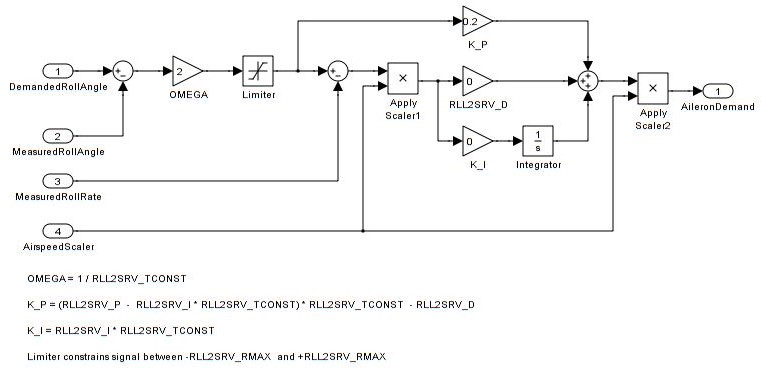
\includegraphics[width=\linewidth]{figs/roll_control_loop.jpg}
  \caption{Roll control loop.}
  \label{fig:roll_loop}
\end{figure}

\subsection{Yaw Control}
The Yaw Control loop controls the angle around the Z axis, $\psi$. This is usually used for landing only, and is not used on this aircraft on airplane mode. It can, however, be seen on Figure \ref{fig:yaw_loop}.
Like the D and I terms on the roll axis, the controller's output is again scaled with the square of the \textit{AirspeedScaler} factor.
%\todo{dafuq?}

\begin{figure}[H]
\centering
  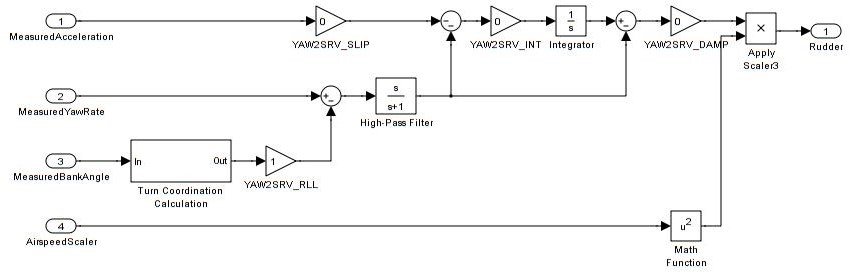
\includegraphics[width=\linewidth]{figs/yaw_control_loop.jpg}
  \caption{Yaw control loop.}
  \label{fig:yaw_loop}
\end{figure}

\subsection{Navigation: L1 Controller}

%S. Park, J. Deyst, and J. P. How, "A New Nonlinear Guidance Logic for
%Trajectory Tracking," Proceedings of the AIAA Guidance, Navigation and
%Control Conference, Aug 2004. AIAA-2004-4900.
%
%
Since a fixed-wing aircraft usually can't fly in-place, waypoints can be used in two general ways, the aircraft can fly around it in circles, or hit it and then follow to the next one.

In order to circle it, a PD controller is used with a feed-forward centripetal force.



